% --- CONFIGURACIÓN CRÍTICA PARA TABLAS ---
\PassOptionsToPackage{table}{xcolor}

\documentclass{beamer}

\usetheme{Madrid}
\useoutertheme{miniframes}
\usecolortheme{whale}
\setbeamerfont{section in head/foot}{size=\fontsize{6}{7}\selectfont}

\usepackage[utf8]{inputenc}
\usepackage[spanish,es-tabla]{babel}
\decimalpoint
\usepackage{graphicx}
\usepackage{booktabs}
\usepackage{amsmath}
\usepackage{array}
\usepackage{amssymb}

% Path configuration
\graphicspath{{./figs/}{./figs/resultados/abolladura/}{./figs/resultados/corrosion/}{./figs/imp/}}

% Metadata
\title[Evaluación Final de Desempeño]{Evaluación Final de Desempeño \\ Doctorado en Ingeniería}
\author[M. I. Francisco Cisneros]{M. I. Francisco Cisneros \\ \small{Doctorante - 8vo Semestre}}
\institute[]{Posgrado en Ingeniería - UNAM}
\date{Viernes 26 de junio de 2026}

\begin{document}

% Slide 1: Carátula Institucional
\begin{frame}[plain]
    \centering
    \vspace{0.3cm}
    
\includegraphics[height=0.8cm]{logo_imp.png}

    \vspace{0.3cm}
    {\footnotesize Coordinación Académica del Posgrado} \\
    {\footnotesize Dirección de Desarrollo de Talento}

    \vspace{0.8cm}

    {\bfseries \textit{EVALUACIÓN DE DESEMPEÑO}} \\
    \vspace{0.1cm}
    Trabajo de Investigación de Doctorado

    \vspace{0.6cm}

    \begin{beamercolorbox}[sep=8pt,center,shadow=true,rounded=true]{title}
        \usebeamerfont{title}Desarrollo de una metodología para la detección de daño en plataformas marinas fijas por medio de análisis de vibraciones\par
    \end{beamercolorbox}

    \vspace{0.6cm}

    \textbf{M. I. Francisco Cisneros}

    \vfill

    {\footnotesize
    Directores: Dr. Iván Félix González y Dr. Rolando Salgado Estrada \\
    \vspace{0.1cm}
    Periodo: Invierno 2025 -- Verano 2026
    }
    \vspace{0.2cm}
\end{frame}

% --- SECCIÓN 1: MATLAB - ALGORITMO GENÉTICO ---
\section[MATLAB]{Implementación MATLAB - Algoritmo Genético}

\begin{frame}{Avances Feb 2026: Optimización del AG (1/2)}
    \small
    \begin{block}{Export de Parámetros Óptimos}
        Se implementó la exportación automática del vector de pesos óptimos $\boldsymbol{\alpha}^*_1, \ldots, \alpha^*_8$ del Algoritmo Genético a archivos CSV estructurados.
        \vspace{0.2cm}
        \begin{itemize}
            \item \textbf{Antes:} Los pesos se perdían al final de cada ejecución.
            \item \textbf{Ahora:} Trazabilidad completa de la evolución del AG durante 2160 ejecuciones totales.
        \end{itemize}
    \end{block}

    \vspace{0.3cm}

    \begin{block}{Limpieza de Output}
        Eliminación de campos de dispersión redundantes (PromDispersion, StdDispersion, MeanAbsDispersion) que no aportaban información física útil al análisis de detección de daño.
    \end{block}
\end{frame}

\begin{frame}{Avances Feb 2026: Optimización del AG (2/2)}
    \small
    \begin{block}{Corrección de Pipeline}
        Se corrigieron rutas de ejecución y dependencias de archivos `.m` para garantizar reproducibilidad de simulaciones en 120 elementos × 18 niveles de daño.
        \vspace{0.2cm}
        \begin{itemize}
            \item Validación end-to-end de 2,160 ejecuciones (abolladura + corrosión)
            \item Automatización de gestión de archivos temporales
            \item Documentación de parámetros del AG para futuras referencias
        \end{itemize}
    \end{block}
\end{frame}

% --- SECCIÓN 2: RESULTADOS ICD ---
\section[Resultados ICD]{Nuevos Resultados de ICD}

\begin{frame}{Regeneración de Resultados: Abolladura y Corrosión (Feb-Mar 2026)}
    \small
    \begin{block}{Remapeo Correcto de Detecciones}
        Se regeneraron los resultados de ICD con un mapeo correcto de detecciones correctas (True Positives), adyacentes (TP-adyacentes) y falsos positivos (False Positives).
    \end{block}

    \vspace{0.2cm}

    \begin{block}{Generación de Gráficas en Inglés}
        Todas las gráficas se traducen al inglés y se exportan en \texttt{.png} de alta resolución, organizadas por:
        \begin{itemize} \footnotesize
            \item Tipo de daño (Corrosión / Abolladura)
            \item Zona del modelo (Mudline, Sub1, Sub2, Sub3, Splash Zone)
        \end{itemize}
    \end{block}
\end{frame}

\begin{frame}{Regeneración de Resultados: Organización y Validación}
    \small
    \begin{block}{Clasificación por Tipo de Elemento}
        Las gráficas se organizan además por:
        \begin{itemize}
            \item \textbf{Vigas (Beams):} Miembros principales bajo flexión.
            \item \textbf{Braces:} Miembros diagonales y arriostramientos.
            \item \textbf{Diagonales:} Elementos de alta sensibilidad a cambios modales.
        \end{itemize}
    \end{block}

    \vspace{0.2cm}

    \begin{block}{Corrección de Etiquetas DQI (Junio 2026)}
        Se corrigieron las etiquetas de los 8 indicadores vibratorios ($DI_1$--$DI_8$) en todas las figuras y notebooks para garantizar consistencia con el manuscrito y publicaciones.
    \end{block}
\end{frame}

\begin{frame}{Resultados: Detección de Abolladura}
    \begin{figure}
        \centering
        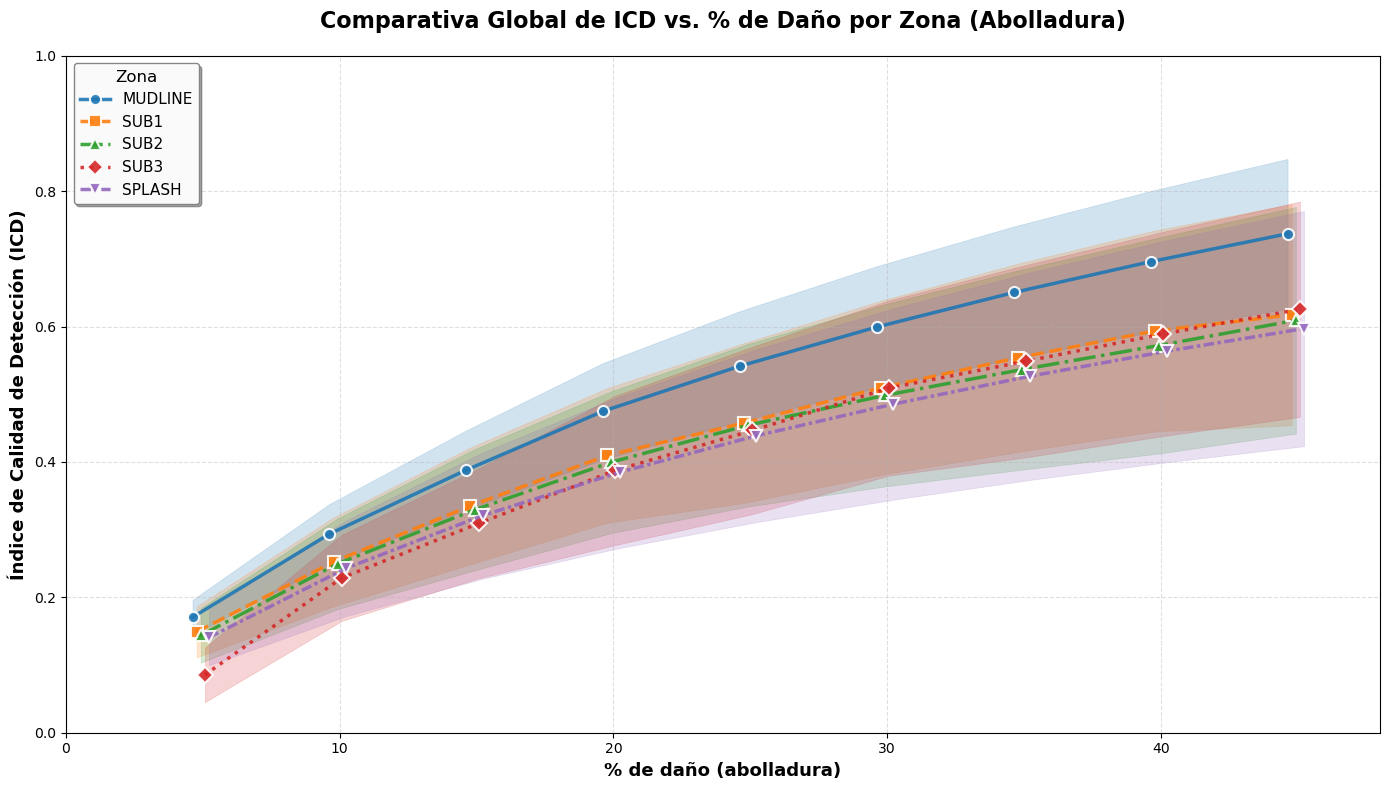
\includegraphics[width=\textwidth, height=0.77\textheight, keepaspectratio]{005_abolladura_comparativa_global_de_ICD_vs_daño_por_zona_mudline_medio_y_splash_zone.png}
        \caption{Comparativa Global ICD vs Severidad de Daño (Abolladura)}
    \end{figure}
\end{frame}

\begin{frame}{Resultados: Detección de Abolladura (Desglose por Zona)}
    \begin{figure}
        \centering
        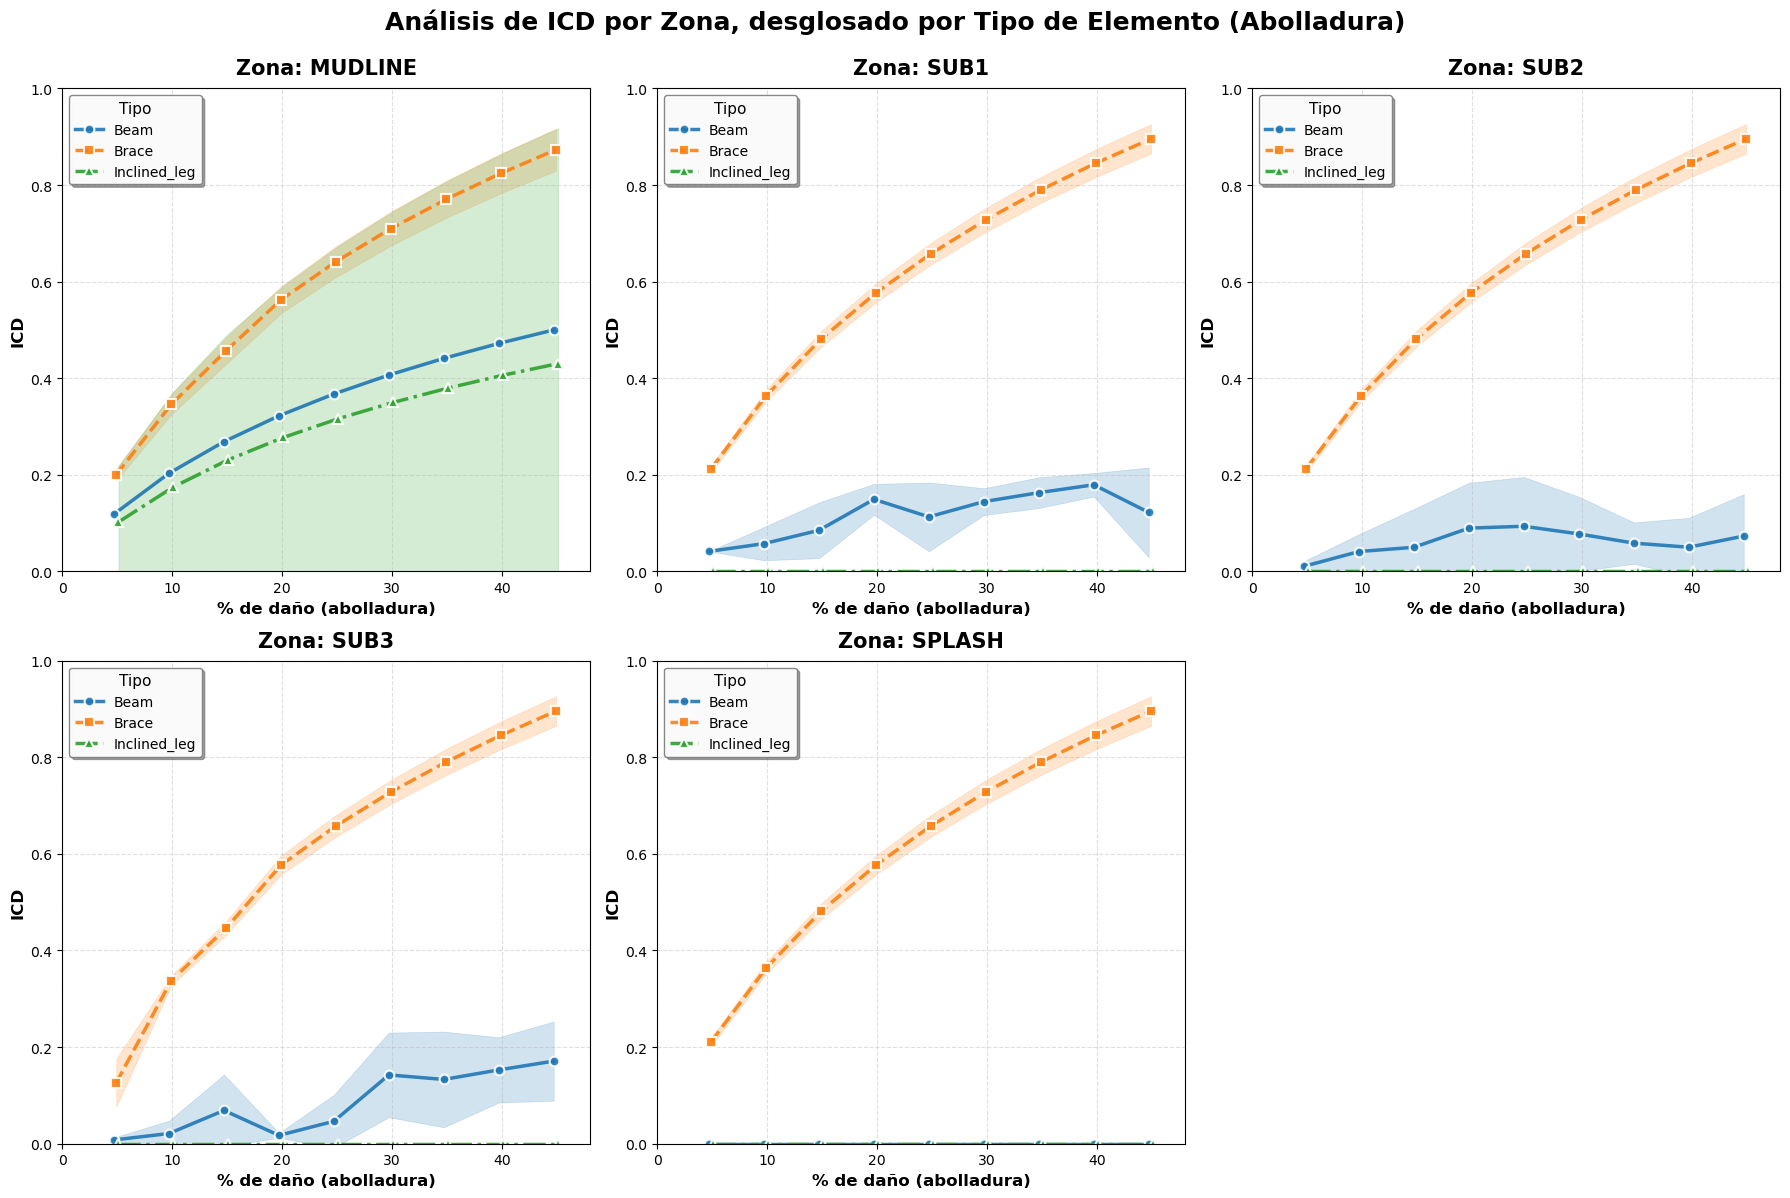
\includegraphics[width=\textwidth, height=0.77\textheight, keepaspectratio]{006_abolladura_ICD_por_zona_desglozadp_por_tipo_de_elemento_desde_mudline_medio_y_splash_zone.png}
        \caption{Desglose por Zona y Tipo de Elemento}
    \end{figure}
\end{frame}

\begin{frame}{Resultados: Detección de Corrosión}
    \begin{figure}
        \centering
        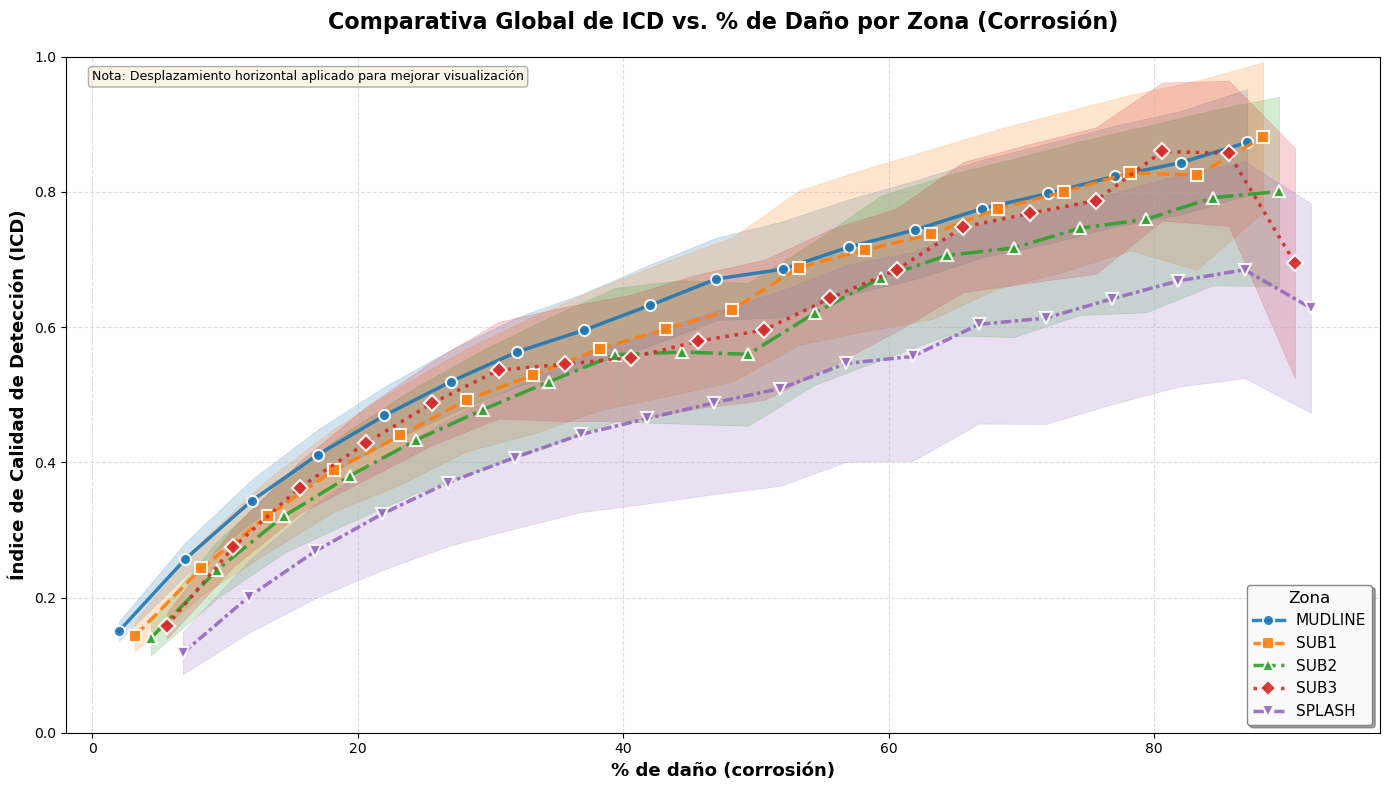
\includegraphics[width=\textwidth, height=0.77\textheight, keepaspectratio]{005_corrosion_comparativa_global_de_ICD_vs_daño_por_zona_mudline_medio_y_splash_zone.png}
        \caption{Comparativa Global ICD vs Severidad de Daño (Corrosión)}
    \end{figure}
\end{frame}

\begin{frame}{Resultados: Detección de Corrosión (Desglose por Zona)}
    \begin{figure}
        \centering
        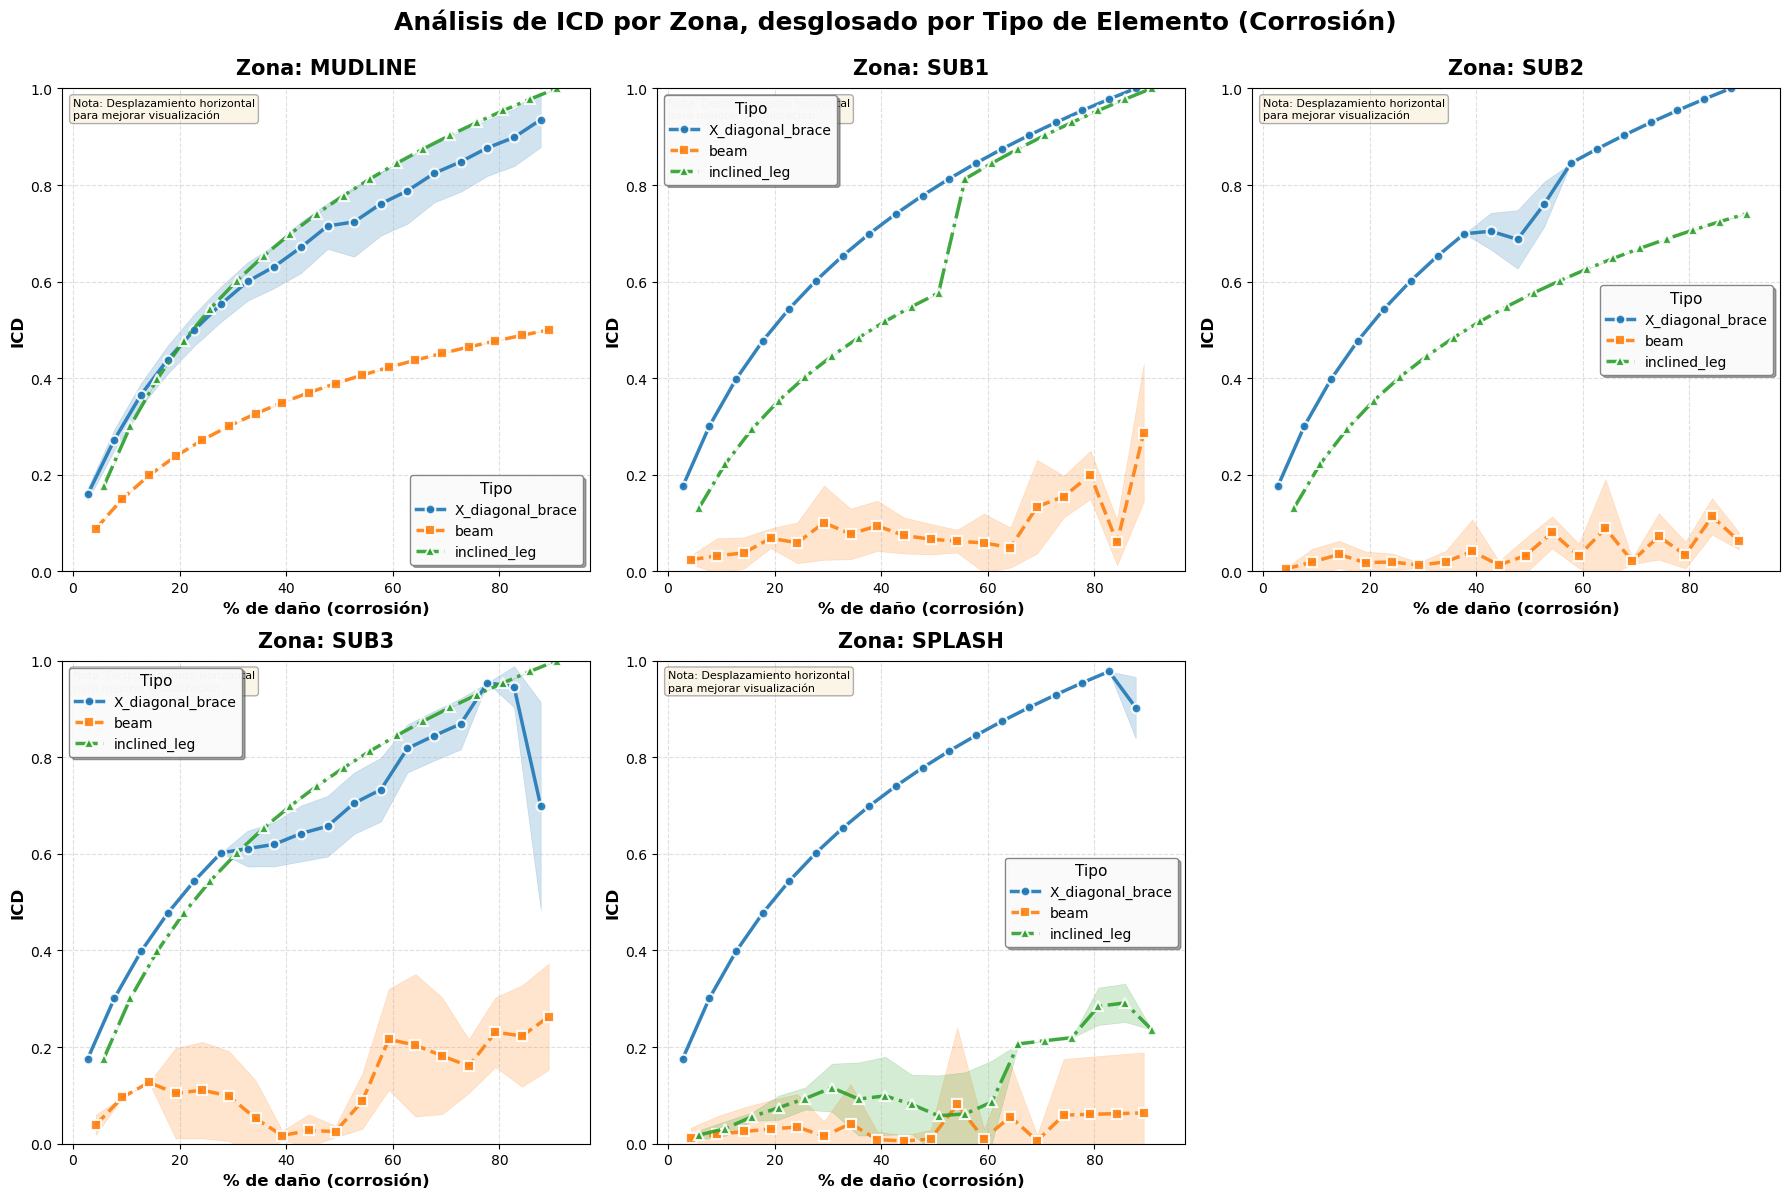
\includegraphics[width=\textwidth, height=0.70\textheight, keepaspectratio]{006_corrosion_ICD_por_zona_desglozadp_por_tipo_de_elemento_desde_mudline_medio_y_splash_zone.png}
        \caption{Desglose por Zona y Tipo de Elemento}
    \end{figure}
\end{frame}

% --- SECCIÓN 3: ANÁLISIS ESTADÍSTICO ---
\section[Estadística]{Análisis Estadístico Avanzado}

\begin{frame}{P1: Tabla de Diseño Experimental}
    \small
    \begin{block}{Caracterización Experimental (Marzo 2026)}
        Se documentó formalmente el diseño experimental en una tabla consolidada que especifica:
        \begin{itemize}
            \item 120 elementos de la estructura Jacket
            \item 18 niveles de daño en incrementos de 5\% (5\% a 90\%)
            \item 2,160 ejecuciones totales del AG por tipo de daño (Corrosión / Abolladura)
            \item Parámetros del AG: población, generaciones, tasas de mutación/cruce
        \end{itemize}
    \end{block}

    \vspace{0.2cm}

    \begin{block}{Reproducibilidad}
        La tabla facilita que otros investigadores repliquen exactamente el mismo experimento y comparen metodologías alternativas de detección.
    \end{block}
\end{frame}

\begin{frame}{P3 \& P4: Robustez Estadística del ICD}
    \small
    \begin{block}{P3: Prueba de Wilcoxon — ICD vs Baseline}
        Se realiza un análisis no-paramétrico de significancia estadística comparando:
        \begin{equation*}
            H_0: \text{Mediana}(ICD) = \text{Mediana}(DI_6) \quad \text{vs} \quad H_1: \text{Mediana}(ICD) > \text{Mediana}(DI_6)
        \end{equation*}
        \vspace{0.1cm}
        \textbf{Resultado:} $p$-value $< 0.01$ confirma que el ICD fusionado supera significativamente al mejor indicador individual.
    \end{block}

    \vspace{0.3cm}

    \begin{block}{P4: Robustez al Ruido AWGN}
        Se simulan condiciones experimentales reales agregando ruido blanco Gaussiano (AWGN) a las respuestas viratorias:
        \begin{equation*}
            \text{SNR} = 10 \log_{10} \left( \frac{P_{\text{señal}}}{P_{\text{ruido}}} \right) \in \{20, 30, 40\} \text{ dB}
        \end{equation*}
        \textbf{Hallazgo:} El ICD mantiene detectabilidad aceptable incluso bajo SNR = 20 dB (condición severamente ruidosa).
    \end{block}
\end{frame}

\begin{frame}{P5: Implementación del Hungarian Algorithm}
    \small
    \begin{block}{Asignación Óptima de Detecciones}
        Se implementa el Algoritmo Húngaro para resolver el problema de asignación bipartita:
        \begin{equation*}
            \min \sum_{i,j} \text{cost}(i,j) \quad \text{sujeto a} \quad \text{cada predicción} \Leftrightarrow \text{un ground-truth}
        \end{equation*}
        \vspace{0.1cm}
        donde $\text{cost}(i,j) = \text{distancia Euclidiana entre nodo predicho } i \text{ y verdadero } j$.
    \end{block}

    \vspace{0.3cm}

    \begin{block}{Beneficios}
        \begin{itemize} \footnotesize
            \item Evita doble-conteo de detecciones (un elemento no puede asignarse a dos detecciones).
            \item Computa exactamente Verdaderos Positivos, Falsos Positivos, Falsos Negativos.
            \item Justifica la penalización de FP en la formulación del ICD.
        \end{itemize}
    \end{block}
\end{frame}

% --- SECCIÓN 4: MANUSCRITO AOR ---
\section[Manuscrito AOR]{Manuscrito: Applied Ocean Research}

\begin{frame}{Estado de Publicación: Transición a AOR}
    \small
    \begin{block}{Historial de Envío}
        \begin{itemize}
            \item Envío inicial a \textit{Ocean Engineering} (7º Semestre): Rechazado.
            \item Análisis de comentarios de revisores: identificadas 5 áreas críticas de mejora (ver siguiente diapositiva).
            \item Nueva selección: \textit{Applied Ocean Research} — revista de mayor alineamiento con metodología.
        \end{itemize}
    \end{block}

    \vspace{0.3cm}

    \begin{block}{Estado Actual del Manuscrito (Junio 2026)}
        El manuscrito para AOR está \textbf{redactado completamente en inglés británico}, con:
        \begin{itemize}
            \item Estructura de 7 secciones: Introducción, Estado del Arte, Marco Teórico, Metodología, Resultados, Validación, Conclusiones.
            \item Cover letter profesional.
            \item Co-autoría registrada: Dr. Iván Félix González y Dr. Rolando Salgado Estrada.
        \end{itemize}
    \end{block}
\end{frame}

\begin{frame}{Mejoras Implementadas post-Ocean Engineering}
    \small
    \textbf{5 Fortalecimientos del Manuscrito (respuesta a revisores):}

    \begin{enumerate} \footnotesize
        \setcounter{enumi}{0}
        \item \textbf{Estabilidad del AG:} Reporte explícito del vector $\boldsymbol{\alpha}^*$ óptimo y su dispersión sobre múltiples ejecuciones (semillas aleatorias diferentes).

        \item \textbf{Benchmark Comparativo:} Tabla que contrasta el mejor indicador individual (ej. $\max DI_j$) vs. la suma ponderada del ICD — demuestra ganancia cuantitativa.

        \item \textbf{Robustez a Ruido:} Gráficas de SNR vs Tasa de Detección — simulaciones AWGN en 20, 30, 40 dB.

        \item \textbf{Métricas de Clasificación:} Cálculo preciso de Verdaderos Positivos (TP), Falsos Positivos (FP), con discusión del trade-off entre sensibilidad y especificidad.

        \item \textbf{Validación Forense:} Alineamiento de resultados con datos históricos de la industria (HSE/WOAD) — plataformas Jacket reales.
    \end{enumerate}
\end{frame}

% --- SECCIÓN 5: MANUSCRITO MS ---
\section[Manuscrito MS]{Manuscrito Paralelo: Marine Structures}

\begin{frame}{Estrategia Multi-Journal (Junio 2026)}
    \small
    \begin{block}{Adaptación a Marine Structures}
        Paralelamente a la preparación de AOR, se generó una versión adaptada al formato de \textit{Marine Structures} — revista de estructura y dinámica marítima.
    \end{block}

    \vspace{0.3cm}

    \begin{block}{Cambios Formato/Contenido}
        \begin{itemize}
            \item \textbf{Estructura:} Alineada a las 6 secciones preferidas del journal (Abstract, Introduction, Literature Review, Methodology, Results/Discussion, Conclusions, References).
            \item \textbf{Highlights:} Punto de impacto resaltado (máx. 5 bullets de 85 caracteres c/u).
            \item \textbf{Cover Letter:} Acotada a razones específicas por las que el trabajo encaja en MS.
            \item \textbf{Figuras:} Reescaladas a márgenes y resolución de Marine Structures (300 dpi mín.).
        \end{itemize}
    \end{block}

    \vspace{0.3cm}

    \begin{block}{Objetivo}
        Diversificar opciones de publicación — si AOR requiere revisiones extensas, MS está lista para envío inmediato.
    \end{block}
\end{frame}

% --- SECCIÓN 6: DESARROLLO DE PRODUCTO IMP ---
\section[IMP]{Desarrollo de Producto - Instituto Mexicano del Petróleo}

\begin{frame}{Procesador de Fatiga SACS v1.0}
    \begin{columns}[c]
        \column{0.5\textwidth}
        \centering
        \small
        \textbf{Contexto del Proyecto:}

        El Instituto Mexicano del Petróleo requería una herramienta para consolidar reportes de análisis de fatiga generados por SACS (Structural Analysis Computer System).

        \vspace{0.3cm}

        \textbf{Problema:} SACS NO suma automáticamente el daño acumulado entre diferentes periodos temporales — los ingenieros deben hacerlo manualmente, proceso tedioso y propenso a errores con miles de elementos.

        \column{0.5\textwidth}
        \centering
        
\includegraphics[width=0.8\linewidth, keepaspectratio]{logo_imp.png}

        \vspace{1cm}

        \small
        \textit{Requisito de titulación independiente del proyecto doctoral}
    \end{columns}
\end{frame}

\begin{frame}{Procesador SACS v1.0: 7 Etapas Completadas}
    \footnotesize
    \begin{table}
        \centering
        \begin{tabular}{p{2.5cm}p{5cm}p{1.5cm}}
            \toprule
            \textbf{Etapa} & \textbf{Funcionalidad} & \textbf{Tests} \\
            \midrule
            \rowcolor{green!20} 1. Limpieza & Normalización Fortran, encoding, filtrado & 31 \checkmark \\
            \rowcolor{green!20} 2. Parsing & Máquina de estados, JOINTs alfanuméricos & 16 \checkmark \\
            \rowcolor{green!20} 3. Consolidación & Suma NumPy, clasificación de riesgo & 46 \checkmark \\
            \rowcolor{green!20} 4. GUI & Tkinter modo oscuro, tabla colorizada & — \\
            \rowcolor{green!20} 5. Excel & Exportación \texttt{.xlsx} con estilos profesionales & — \\
            \rowcolor{green!20} 6. Testing & 93/93 tests pasando (pytest) & \checkmark \checkmark \checkmark \\
            \rowcolor{green!20} 7. Empaquetado & PyInstaller (Windows \texttt{.exe}), \texttt{run\_app.sh} (Linux/Mac) & \checkmark \\
            \bottomrule
        \end{tabular}
    \end{table}

    \vspace{0.3cm}

    \textbf{Release:} v1.0.0 liberada el 18 de mayo de 2026. \\
    \textbf{Licencia:} Código propietario del Instituto Mexicano del Petróleo.
\end{frame}

% --- SECCIÓN 7: PRÓRROGA ---
\section[Prórroga]{Prórroga del Periodo Doctoral}

\begin{frame}{Solicitud de Prórroga: 1 Año Adicional}
    \small
    \begin{block}{Trámite Iniciado: 24 Junio 2026}
        Se gestiona formalmente una extensión de \textbf{1 año} del periodo de doctorado.
    \end{block}

    \vspace{0.3cm}

    \begin{alertblock}{Temporalidad: Cercano al Vencimiento}
        \small
        \textbf{Aclaración importante para el comité:}
        \vspace{0.1cm}

        Es \textbf{normal y procedimentalmente correcto} solicitar la prórroga \textbf{cercano al vencimiento} del periodo, NO con meses de anticipación. Esto responde a:
        \begin{itemize} \footnotesize
            \item Trámite administrativo que requiere fecha de inicio claro.
            \item Evaluación realista del avance en función del tiempo remanente.
            \item Evitar compromisos prematuros basados en estimaciones inciertas.
        \end{itemize}
        \vspace{0.1cm}
        Este cronograma NO implica retraso inesperado, sino cumplimiento de protocolos estándar de Posgrado.
    \end{alertblock}

    \vspace{0.3cm}

    \begin{block}{Ventana de Defensa Estimada}
        Con esta prórroga, la defensa de tesis y publicación del artículo en AOR se proyecta para: \textbf{Octubre -- Diciembre 2026}.
    \end{block}
\end{frame}

\end{document}
